\begingroup
\setlength{\abovedisplayskip}{6pt}
\setlength{\belowdisplayskip}{6pt}
\setlength{\abovedisplayshortskip}{4pt}
\setlength{\belowdisplayshortskip}{4pt}
\setlength{\intextsep}{6pt}

The beam calculation uses SI units, while the response plots report displacement in millimetres. I idealize the leaf spring as a simply supported beam with a concentrated load at its center because this matches the two spring-eye supports and the center displacement shown in the model. Therefore, the corresponding center deflection is

\[
\delta=\frac{PL^3}{48EI},
\qquad
k=\frac{P}{\delta}=\frac{48EI}{L^3}.
\]

This support condition is important because a cantilever model would produce a different stiffness.

\textbf{B.4.1. Input data.}

{ % do not increment counter
\begin{center}\small\begin{tabular}{@{}lrl@{}}
\toprule\noalign{}
Quantity & Value & Unit \\
\midrule\noalign{}
$L$ & 0.830 & m \\
$b$ & 0.065 & m \\
$h$ & 0.003 & m \\
$E$ & 200 & GPa \\
$m$ & 457 & kg \\
$u_0$ & 125 & mm \\
$\dot{u}_0$ & 0 & mm/s \\
$\zeta_{\mathrm{H}}$ & 0.25 & 1 \\
$\zeta_{\mathrm{W}}$ & 0.10 & 1 \\
$g$ & 9.81 & m/s$^2$ \\
\bottomrule\end{tabular}\end{center}
}

For vertical bending about the horizontal centroidal axis, the section dimension perpendicular to that axis is $h$, so $h$ is cubed in the second moment of area.

\[
I=\frac{bh^3}{12}
 =\frac{(0.065)(0.003)^3}{12}
 =1.4625\times10^{-10}\ \mathrm{m^4}
 =146.25\ \mathrm{mm^4}.
\]

\[
\boxed{I=1.4625\times10^{-10}\ \mathrm{m^4}=146.25\ \mathrm{mm^4}}
\qquad\text{(B.4.2)}
\]

Multiplying the section property by the elastic modulus gives the flexural rigidity.

\[
EI=(200\times10^9)(1.4625\times10^{-10})
 =29.25\ \mathrm{N\,m^2}.
\]

\[
\boxed{EI=29.25\ \mathrm{N\,m^2}}
\qquad\text{(B.4.3)}
\]

Substitution into the simply supported center-load relation gives the equivalent spring constant.

\[
k=\frac{48EI}{L^3}
 =\frac{48(29.25)}{(0.830)^3}
 =2455.46\ \mathrm{N/m}.
\]

\[
\boxed{k=2.455\times10^3\ \mathrm{N/m}}
\qquad\text{(B.4.4)}
\]

The undamped natural frequency follows from the mass and equivalent stiffness. Its cyclic frequency is found by dividing by $2\pi$.

\[
\omega_n=\sqrt{\frac{k}{m}}=\sqrt{\frac{2455.46}{457}}=2.31797\ \mathrm{rad/s},
\qquad
f_n=\frac{\omega_n}{2\pi}=0.368917\ \mathrm{Hz}.
\]

\[
\boxed{\omega_n=2.32\ \mathrm{rad/s},\qquad f_n=0.3689\ \mathrm{Hz}}
\qquad\text{(B.4.5)}
\]

Critical damping makes the characteristic-equation roots coincide. Therefore,

\[
c_{\mathrm{cr}}=2\sqrt{mk}=2\sqrt{(457)(2455.46)}
 =2118.63\ \mathrm{N\,s/m}.
\]

\[
\boxed{c_{\mathrm{cr}}=2.119\times10^3\ \mathrm{N\,s/m}}
\qquad\text{(B.4.6)}
\]

For the original damper, the specified damping ratio is $\zeta_{\mathrm{H}}=0.25$. The physical damping is the damping ratio multiplied by the critical value.

\[
c_{\mathrm{H}}=\zeta_{\mathrm{H}}c_{\mathrm{cr}}
 =(0.25)(2118.63)=529.657\ \mathrm{N\,s/m}.
\]

\[
\boxed{\zeta_{\mathrm{H}}=0.250,\qquad c_{\mathrm{H}}=529.7\ \mathrm{N\,s/m}}
\qquad\text{(B.4.7)}
\]

Because $\zeta_{\mathrm{H}}<1$, the original system is underdamped. Its damped frequency and cyclic frequency are

\[
\omega_{d,\mathrm{H}}=\omega_n\sqrt{1-\zeta_{\mathrm{H}}^2}
 =2.31797\sqrt{1-0.25^2}=2.24437\ \mathrm{rad/s},
\qquad
f_{d,\mathrm{H}}=\frac{\omega_{d,\mathrm{H}}}{2\pi}=0.357202\ \mathrm{Hz}.
\]

\[
\boxed{\omega_{d,\mathrm{H}}=2.24\ \mathrm{rad/s},\qquad f_{d,\mathrm{H}}=0.3572\ \mathrm{Hz}}
\qquad\text{(B.4.8)}
\]

The time for one damped oscillation is the damped period.

\[
\tau_{d,\mathrm{H}}=\frac{2\pi}{\omega_{d,\mathrm{H}}}
 =\frac{2\pi}{2.24437}=2.79954\ \mathrm{s}.
\]

\[
\boxed{\tau_{d,\mathrm{H}}=2.80\ \mathrm{s}}
\qquad\text{(B.4.9)}
\]

Defining the decay rate as $\alpha_{\mathrm{H}}=\zeta_{\mathrm{H}}\omega_n=0.579493\ \mathrm{s^{-1}}$ gives the characteristic roots

\[
s_{1,2}=-\alpha_{\mathrm{H}}\pm i\omega_{d,\mathrm{H}}
 =-0.579493\pm i\,2.24437\ \mathrm{s^{-1}}.
\]

For the zero-velocity initial condition, the exponential constants are obtained from the trigonometric coefficients $A=u_0$ and $B=\alpha_{\mathrm{H}}u_0/\omega_{d,\mathrm{H}}$. Since $A=C_1+C_2$ and $B=i(C_1-C_2)$,

\[
C_1=\frac{A-iB}{2}=62.500-16.137i\ \mathrm{mm},
\qquad
C_2=\frac{A+iB}{2}=62.500+16.137i\ \mathrm{mm}.
\]

\[
\boxed{
\begin{aligned}
s_1&=-0.5795+i\,2.2444\ \mathrm{s^{-1}},\qquad
s_2=-0.5795-i\,2.2444\ \mathrm{s^{-1}},\\
C_1&=62.50-16.14i\ \mathrm{mm},\qquad
C_2=62.50+16.14i\ \mathrm{mm}
\end{aligned}}
\qquad\text{(B.4.10)}
\]

The real trigonometric coefficients are

\[
A=u_0=125.0\ \mathrm{mm},
\qquad
B=\frac{\alpha_{\mathrm{H}}u_0}{\omega_{d,\mathrm{H}}}=32.2749\ \mathrm{mm}.
\]

Writing the harmonic part as a single sine function gives $A=C\sin\phi$ and $B=C\cos\phi$. Therefore,

\[
C=\sqrt{A^2+B^2}=129.099\ \mathrm{mm},
\qquad
\phi=\operatorname{atan2}(A,B)=1.31812\ \mathrm{rad}.
\]

The displacement response for the original damper is consequently

\[
u_{\mathrm{H}}(t)=129.099e^{-0.579493t}\sin(2.24437t+1.31812)\ \mathrm{mm}.
\]

\[
\boxed{
\begin{aligned}
A&=125.0\ \mathrm{mm},& B&=32.27\ \mathrm{mm},\\
C&=129.1\ \mathrm{mm},& \phi&=1.318\ \mathrm{rad}
\end{aligned}}
\qquad\text{(B.4.11)}
\]

At one damped period, the sine and cosine terms return to their initial values. The displacement is therefore the initial displacement multiplied by the decay factor for one period.

\[
t_{1,\mathrm{H}}=\tau_{d,\mathrm{H}}=2.79954\ \mathrm{s},
\qquad
u_{1,\mathrm{H}}=u_{\mathrm{H}}(t_{1,\mathrm{H}})
 =u_0e^{-\alpha_{\mathrm{H}}t_{1,\mathrm{H}}}=24.680\ \mathrm{mm}.
\]

\[
\boxed{t_{1,\mathrm{H}}=2.80\ \mathrm{s},\qquad u_{1,\mathrm{H}}=24.68\ \mathrm{mm}}
\qquad\text{(B.4.12)}
\]

The displacement magnitude defining the 2\% band is

\[
u_{0.02}=0.02u_0=0.02(125)=2.50\ \mathrm{mm}.
\]

\[
\boxed{u_{0.02}=2.50\ \mathrm{mm}}
\qquad\text{(B.4.13)}
\]

The largest response is the initial displacement, so $|u|_{\max}=125\ \mathrm{mm}$ at $t=0$. The last extremum with magnitude greater than $u_{0.02}$ occurs at approximately $t=5.599\ \mathrm{s}$, where $u=4.873\ \mathrm{mm}$. Solving the descending branch for $u(t)=u_{0.02}$ gives the final entry into the 2\% band at $t_s=6.090\ \mathrm{s}$. All later extrema have magnitude below $2.50\ \mathrm{mm}$.

\[
\boxed{|u|_{\max}=125.0\ \mathrm{mm}\quad\text{at }t=0}
\qquad\text{(B.4.14.a)}
\]

\[
\boxed{u(t_{1,\mathrm{H}})=24.68\ \mathrm{mm}\quad\text{at }t_{1,\mathrm{H}}=2.80\ \mathrm{s}}
\qquad\text{(B.4.14.b)}
\]

\[
\boxed{t_{s,\mathrm{H}}=6.09\ \mathrm{s},\qquad u_{\mathrm{H}}(t_{s,\mathrm{H}})=+2.50\ \mathrm{mm}}
\qquad\text{(B.4.14.c)}
\]

\begin{figure}[H]
\centering
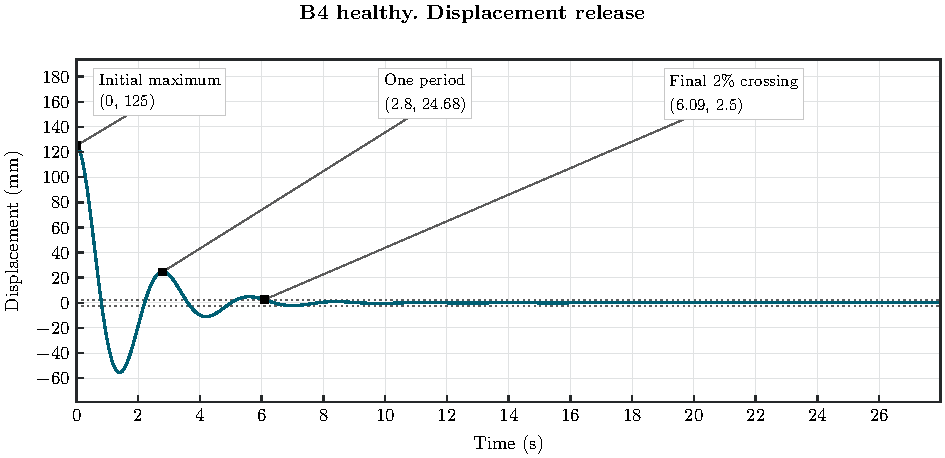
\includegraphics[width=0.95\linewidth,height=0.30\textheight,keepaspectratio,alt={B.4. Original damper response for ten oscillations with the initial maximum, one-period response, and final 2 percent crossing marked.}]{figures/generated/solutions/B4_healthy.pdf}
\caption{B.4.14.a-b-c. Original damper response for ten oscillations.}
\end{figure}

\textbf{B.4.15. Discussion.}

The original damper produces a decaying underdamped response. The damped period is $2.80\ \mathrm{s}$, and the displacement after one period is reduced from $125\ \mathrm{mm}$ to $24.68\ \mathrm{mm}$. The response remains oscillatory, but its extrema decrease because the envelope is $Ce^{-\alpha_{\mathrm{H}}t}$. The final permanent entry into the 2\% band occurs at $6.09\ \mathrm{s}$.

The calculated static displacement under the apportioned weight is

\[
\delta_{\mathrm{static}}=\frac{mg}{k}
 =\frac{(457)(9.81)}{2455.46}=1.826\ \mathrm{m}.
\]

This is larger than the beam span and much larger than the prescribed $125\ \mathrm{mm}$ initial displacement. The value indicates that the uniform single-beam model is a formal linear approximation. A physical suspension would require the actual leaf-spring stack, support geometry, preload, and available travel.

For the worn damper, the stiffness and mass do not change. Consequently, $I$, $EI$, $k$, $\omega_n$, $f_n$, and $c_{\mathrm{cr}}$ remain unchanged. Using $\zeta_{\mathrm{W}}=0.10$ therefore gives the new damping and decay rate

\[
c_{\mathrm{W}}=\zeta_{\mathrm{W}}c_{\mathrm{cr}}=211.863\ \mathrm{N\,s/m},
\qquad
\alpha_{\mathrm{W}}=\zeta_{\mathrm{W}}\omega_n=0.231797\ \mathrm{s^{-1}}.
\]

The smaller damping ratio gives

\[
\omega_{d,\mathrm{W}}=\omega_n\sqrt{1-\zeta_{\mathrm{W}}^2}=2.30635\ \mathrm{rad/s},
\qquad
f_{d,\mathrm{W}}=0.367068\ \mathrm{Hz},
\]

\[
\tau_{d,\mathrm{W}}=\frac{2\pi}{\omega_{d,\mathrm{W}}}=2.72429\ \mathrm{s}.
\]

The worn-damper roots and exponential constants are

\[
s_{1,2}^{\mathrm{W}}=-0.231797\pm i\,2.30635\ \mathrm{s^{-1}},
\qquad
C_1^{\mathrm{W}}=62.500-6.281i\ \mathrm{mm},
\qquad
C_2^{\mathrm{W}}=62.500+6.281i\ \mathrm{mm}.
\]

The corresponding real coefficients are

\[
A_{\mathrm{W}}=125.0\ \mathrm{mm},
\qquad
B_{\mathrm{W}}=12.563\ \mathrm{mm},
\qquad
C_{\mathrm{W}}=125.630\ \mathrm{mm},
\qquad
\phi_{\mathrm{W}}=1.47063\ \mathrm{rad}.
\]

Thus, the worn-damper response is

\[
u_{\mathrm{W}}(t)=125.630e^{-0.231797t}\sin(2.30635t+1.47063)\ \mathrm{mm}.
\]

The response after one period and the final permanent 2\% crossing are

\[
t_{1,\mathrm{W}}=\tau_{d,\mathrm{W}}=2.72429\ \mathrm{s},
\qquad
u_{1,\mathrm{W}}=u_0e^{-\alpha_{\mathrm{W}}t_{1,\mathrm{W}}}=66.475\ \mathrm{mm},
\]

\[
t_{s,\mathrm{W}}=16.559\ \mathrm{s},
\qquad
u_{\mathrm{W}}(t_{s,\mathrm{W}})=+u_{0.02}=2.50\ \mathrm{mm}.
\]

\[
\boxed{
\begin{aligned}
c_{\mathrm{cr}}&=2118.63\ \mathrm{N\,s/m},& c_{\mathrm{W}}&=211.86\ \mathrm{N\,s/m},\\
\omega_{d,\mathrm{W}}&=2.306\ \mathrm{rad/s},& f_{d,\mathrm{W}}&=0.3671\ \mathrm{Hz},\\
\tau_{d,\mathrm{W}}&=2.724\ \mathrm{s},& s_{1,2}^{\mathrm{W}}&=-0.2318\pm i\,2.306\ \mathrm{s^{-1}},\\
C_1^{\mathrm{W}}&=62.50-6.281i\ \mathrm{mm},& C_2^{\mathrm{W}}&=62.50+6.281i\ \mathrm{mm},\\
A_{\mathrm{W}}&=125.0\ \mathrm{mm},& B_{\mathrm{W}}&=12.56\ \mathrm{mm},\\
C_{\mathrm{W}}&=125.6\ \mathrm{mm},& \phi_{\mathrm{W}}&=1.471\ \mathrm{rad},\\
t_{1,\mathrm{W}}&=2.724\ \mathrm{s},& u_{1,\mathrm{W}}&=66.48\ \mathrm{mm}
\end{aligned}}
\qquad\text{(B.4.16.a)}
\]

\textbf{B.4.16.b. Comparison.} The worn damper has a smaller decay rate, so its oscillations persist longer. Its damped frequency is slightly higher and its period is slightly shorter because reducing damping moves $\omega_d$ closer to $\omega_n$. The one-period displacement increases from $24.68\ \mathrm{mm}$ to $66.48\ \mathrm{mm}$, and the permanent 2\% settling time increases from $6.09\ \mathrm{s}$ to $16.56\ \mathrm{s}$. Both cases have the same initial maximum because they have the same initial displacement.

\begin{figure}[H]
\centering
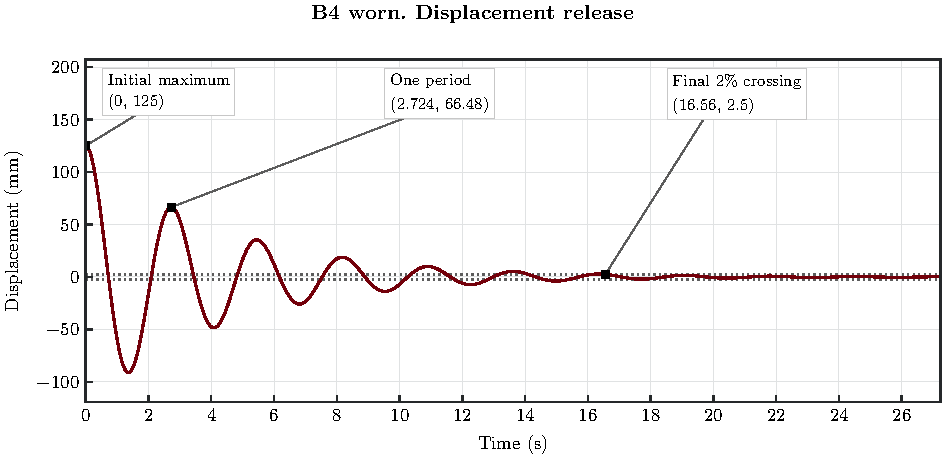
\includegraphics[width=0.95\linewidth,height=0.30\textheight,keepaspectratio,alt={B.4. Worn damper response for ten oscillations with the initial maximum, one-period response, and final 2 percent crossing marked.}]{figures/generated/solutions/B4_worn.pdf}
\caption{B.4.16.a. Worn damper response for ten oscillations.}
\end{figure}

\begin{figure}[H]
\centering
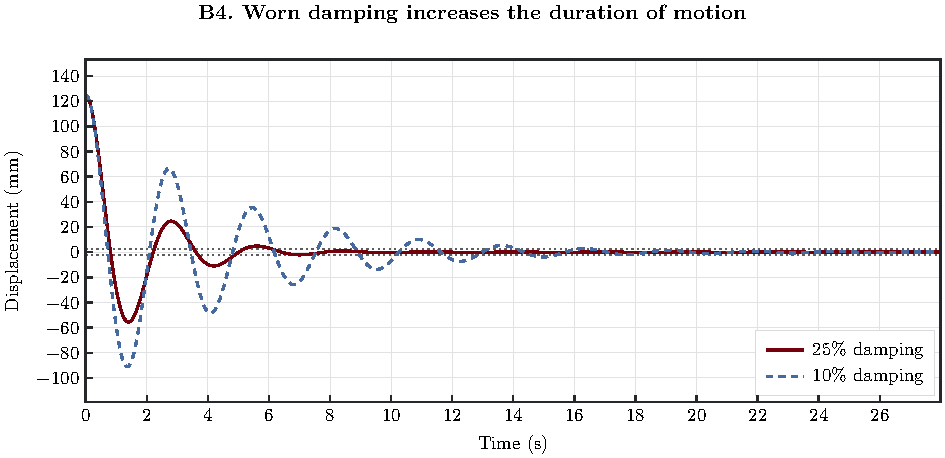
\includegraphics[width=0.95\linewidth,height=0.30\textheight,keepaspectratio,alt={B.4. Comparison of the 25 percent and 10 percent damping responses.}]{figures/generated/solutions/B4_compare.pdf}
\caption{B.4.16.b. Comparison of the original and worn-damper responses.}
\end{figure}

\clearpage
\matlabcaption{MATLAB code used to reproduce the B.4.14 and B.4.16 response plots.}

\lstinputlisting[style=hwmatlab]{matlab/B4.m}
\endgroup
